

\subsection{随机变量的分布}
\title [概率论]{第十讲:随机变量的分布与性质}
\author [张鑫 {\rm Email: xzhangseu@seu.edu.cn} ]{\large 张 鑫}
\institute [东南大学数学学院]{\large \textrm{Email: x.zhang.seu@foxmail.com} \\ \quad  \\
	\large 东南大学 \quad 数学学院 \\
	\vspace{0.3cm}
	%  \trc{公共邮箱: \textrm{zy.prob@qq.com}\\
	%    \hspace{-1.7cm}  密 \qquad 码: \textrm{seu!prob}}
}
\date{}

{ \setbeamertemplate{footline}{}
	\begin{frame}
		\titlepage
	\end{frame}
}

% \begin{frame}[plain]
%   \frametitle{目录}
%   \setcounter{tocdepth}{2}
%   \tableofcontents
% \end{frame}
\addtocounter{framenumber}{-3}  % 目录页不计算页码

\begin{frame}
	\frametitle{分布与分布函数}
	\begin{thm}
		设 $X$ 为 $(\Omega,\mathcal{F},P)$ 上的随机变量,对于 Borel 集 $B$, 定义集函数 $\mathbf{F}(B)$ 如下:
		\begin{eqnarray}\label{eq:rvprob}
			\mathbf{F}(B):=P(X^{-1}(B))=P\circ X^{-1}(B)=P(X\in B)
		\end{eqnarray}
		则 $\mathbf{F}(\cdot)$ 为 $(R,\mathcal{B})$ 上的概率,称之为随机变量 $X$ 的诱导概率测度.
	\end{thm}
	\vspace{0.2cm}
	\pause
	\begin{defi}
		称由 \eqref{eq:rvprob} 式定义在 $(R,\mathcal{B})$ 上的概率测度 $\mathbf{F}(\cdot)$ 为随机变量 $X$ 的概率分布,简称分布.
	\end{defi}
	\pause
	\vspace{0.2cm}
	\begin{itemize}[<+-|alert@+>]
		\item 给定概率空间 $(\Omega,\mathcal{F},P)$,任给随机变量均可在 $(R,\mathcal{B})$ 上诱导出一个概率测度。由此可见,在同一个可测空间上可以定义不同的概率测度.
		\item 对于任意的 $B\in \mathcal{B}$,随机变量 $X$ 落入 $B$ 中的概率可通过 $B$ 的概率测度 $\mathbf{F}(B)$ 得出。这也就是说,概率分布 $\mathbf{F}(\cdot)$ 完全刻画了随机变量 $X$ 取值的概率规律.
	\end{itemize}
\end{frame}


\begin{frame}
	\frametitle{随机变量的分布函数}
	如果我们将 $(R,\mathcal{B})$ 上的测度仅局限于集类 $\mathcal{P}:=\{(-\infty,x],x\in R\}$ 上,由于 $\mathcal{P}$ 中的每条半直线被它的右端点 $x$ 所决定,于是集函数 $F$ 就化为 $R$ 上的点函数.
	\pause
	\begin{defi}
		对于随机变量 $X$ 而言,称 $x$ 的函数
		\begin{eqnarray*}
			F(x):=\mathbf{F}((-\infty,x])=P(X\le x)
		\end{eqnarray*}
		为 $X$ 的概率分布函数或累积分布函数,简称分布函数并记作 $X\sim F (x)$, 有时也以 $F_X (x)$ 表明是 $X$ 的分布函数.
	\end{defi}
	\pause  \begin{rmk}
		也有一些教材按如下方式定义分布函数:
		\begin{eqnarray*}
			F(x):=\mathbf{F}((-\infty,x))=P(X<x)
		\end{eqnarray*}

	\end{rmk}
\end{frame}

\begin{frame}
	\frametitle{分布函数的性质}
	\begin{thm}
		任一分布函数 $F (x)$ 都具有以下三条基本性质
		\begin{enumerate}[<+-|alert@+>]
			\item 单调性非降性:$F (x)$ 是单调非减函数即对任意的 $x_1<x_2$, 有 $F (x_1)\le F (x_2)$;
			\item 右连续性:$F (x)$ 是 $x$ 的右连续函数,即
			      \begin{eqnarray*}
				      F(x_0)=F(x_0+):=\lim_{x\rightarrow x_0+}F(x)
			      \end{eqnarray*}

			\item 规范性:对任意的 $x$ 有,$0\le F (x)\le 1$ 且
			      \begin{eqnarray*}
				      F(-\infty)=\lim_{x\rightarrow-\infty}F(x)=0\\
				      F(+\infty)=\lim_{x\rightarrow +\infty}F(x)=1
			      \end{eqnarray*}
		\end{enumerate}

	\end{thm}
	\pause%
	\begin{rmk}
	在函数论中, 我们一般不从随机变量出发来定义分布函数, 而是直接定义满足上面三条性质的函数为分布函数.
	\end{rmk}

\end{frame}

\begin{frame}
	\frametitle{分布函数性质的证明}
	\begin{enumerate}[<+-|alert@+>]
		\item 对任意的 $x<y$, $F (y)-F (x)=P (x< X\le y)\ge 0$;
		\item 因 $F (x)$ 是单调有界非降函数,所以其任一点 $x_0$ 的右极限 $F (x_0+)$ 必存在,为证其连续性,只需证对单调上下降且收敛至 $x_0$ 的数列 $\{x_n\}$ 有 $\lim_{n\rightarrow\infty} F (x_n)=F (x_0)$ 即可。注意到
		      \begin{eqnarray*}
			      \lim_{n\rightarrow\infty}F(x_n)&=&\pause \lim_{n\rightarrow\infty}P(X\le x_n)=\pause P(\cap_{n=1}^\infty \{X\le x_n\})=\pause P(X\le x_0)\\\pause
			      &=&F(x_0)
		      \end{eqnarray*}


		\item 由 $F$ 的单调性及概率的连续性可知
		      \begin{eqnarray*}
			      F(+\infty)&=&\pause \lim_{n\rightarrow +\infty}F(n)=\lim_{n\rightarrow +\infty}P(X\le n)\\
			      &=&\pause P(\cup_{n=1}^\infty \{X\le n\})=P(X<\infty)=1
		      \end{eqnarray*}
		      \pause  同理可证 $F (-\infty)=0$.

	\end{enumerate}


\end{frame}
% \begin{frame}
%   \frametitle{事件概率的分布函数表示}
%   \begin{itemize}[<+-|alert@+>]
%   \item $P(a<X\le b)=F(b)-F(a)$;
%   \item $P(X=a)=F(a)-F(a-0)$;
%   \item $P(X\ge b)=1-F(b-0)$;
%   \item $P(X>b)=1-F(b)$;
%   \item $P(a<X<b)=F(b-0)-F(a)$;
%   \item $P(a\le X\le b)=F(b)-F(a-0)$;
%   \item $P(a\le X<b)=F(b-0)-F(a-0)$;
%   \item 对于不交区间并 $\cup_{i=1}^n [a_i,b_i)$, $P (X\in \cup_{i=1}^n [a_i,b_i))=\sum_{i=1}^n [F (b_i-0)-F (a_i-0)]$
%   \end{itemize}
% \end{frame}

% \begin{frame}
%   \frametitle{函数成为分布函数的充分条件}
%   \begin{thm}
%     若函数 $F (x)$ 具有以下三条基本性质
%     \begin{enumerate}[<+-|alert@+>]
%     \item 单调性:$F (x)$ 是单调非减函数即对任意的 $x_1<x_2$, 有 $F (x_1)\le F (x_2)$;
%     \item 有界性:对任意的 $x$ 有,$0\le F (x)\le 1$ 且
%       \begin{eqnarray*}
%         F(-\infty)=\lim_{x\rightarrow-\infty}F(x)=0\\
%         F(+\infty)=\lim_{x\rightarrow +\infty}F(x)=1
%       \end{eqnarray*}
%     \item 右连续性:$F (x)$ 是 $x$ 的右连续函数,即
%       \begin{eqnarray*}
%         F(x_0+):=\lim_{x\rightarrow x_0+}F(x)=F(x_0)
%       \end{eqnarray*}
%     \end{enumerate}
%     则 $F (x)$ 必定是某个随机变量的分布函数.
%   \end{thm}
% \end{frame}
\begin{frame}
	\frametitle{事件概率的分布函数表示}
	\begin{itemize}[<+-|alert@+>]
		\item $P(X> b)=1-F(b)$;%\mathbf{F}((b,\infty))$;
		\item $P(a< X\le b)=F(b)-F(a)$;%\mathbf{F}((a,b])$;

		\item $P(X<a)=F(a-)$;%\mathbf{F}((-\infty, a))$;

		\item $P(X=a)=F(a)-F(a-)$;%\mathbf{F}(\{a\})$;
		\item $P(X\ge b)=1-F(b-)$;%\mathbf{F}([b,\infty))$;

		\item $P(a\le X<b)=F(b-)-F(a-)$;%\mathbf{F}([a,b))$;
		\item $P(a\le X\le b)=F(b)-F(a-)$;%\mathbf{F}([a,b])$;
		\item $P(a< X<b)=F(b-)-F(a)$;%\mathbf{F}((a,b))$;
		\item 对于不交区间并: %$\cup_{i=1}^n [a_i,b_i)$,
		$P (X\in \cup_{i=1}^n (a_i,b_i])=\sum_{i=1}^n [F (b_i)-F (a_i)]$;%\mathbf{F}(\cup_{i=1}^n (a_i,b_i])$
		\item 一般的,$P (X\in B)=\int_BdF (x)$.
	\end{itemize}
\end{frame}


\begin{frame}{随机变量与其分布(函数)之间的关系}
\begin{itemize}[<+-|alert@+>]
	\item 分布函数是随机变量最基本的性质,也是对随机变量概率特性最全面的描述。为清晰起见,通常记随机变量 $X$ 的分布函数为 $F_{X}(x)$.
	\item 分布函数和随机变量密不可分. 每个随机变量都有自己的分布函数; 反过来, 每个分布函数都能找到与之相对应的随机变量.
	\item 尽管随机变量与其分布函数密切关联,但是两者间并没有一一对应关系。一个随机变量只能有唯一的分布函数, 不同的随机变量却可能具有相同的分布函数.

\end{itemize}
\pause
\begin{exam}
  (\tc{不同的随机变量有相同的分布}) 考虑随机变量 $X$, 其分布满足
	\[
	P(X=1)=P(X=-1)=\frac{1}{2}.
	\]\pause
	设随机变量 $Y=-X$, 那么 $Y$ 的分布为
	\[
	P(Y=1)=P(Y=-1)=\frac{1}{2}
	\]\pause
	显然, $X$和$Y$的分布函数完全相同, 但明显是两个不同的随机变量.
\end{exam}


\end{frame}

\begin{frame}
	\frametitle{分布函数表示与Borel域上概率测度之间的关系}
\begin{thm}
任给一个定义在 Borel 域 \( \mathcal{B}(\mathbb{R}) \) 上的概率 \( \bar{P} \), 都存在如下定义的分布函数 \( F \) 与之相对应:$	F(x)=\bar{P}((-\infty, x])$. 反过来, 任给一个定义于实数轴上的分布函数 $F$, 都存在定义在 Borel 域 $\mathcal{B}(\mathbb{R})$ 上的概率 $\bar{P}$ 与之相对应.
\end{thm}

\pause

\zheng
第一个结论可直接验证. 由概率的单调性, 若$x_{1} \leqslant x_{2}$, 则
{\small \[\bar{P}\left(\left(-\infty, x_{1}\right]\right) \leqslant \bar{P}\left(\left(-\infty, x_{2}\right]\right)\Rightarrow F\left(x_{1}\right) \leqslant F\left(x_{2}\right),\]}从而得到 $F$ 的单调不减. \pause 再由概率的连续性,
{\small \begin{eqnarray*}
	\lim _{x_{n} \downarrow x}\left(-\infty, x_{n}\right]=(-\infty, x]
	&\Rightarrow&  \lim _{x_{n} \downarrow x} \bar{P}\left(\left(-\infty, x_{n}\right]\right)=\bar{P}((-\infty, x]) \\
	&\Rightarrow&  \lim _{x_{n} \downarrow x} F\left(x_{n}\right)=F(x)
\end{eqnarray*}}%
\pause
定理的第二个结论本质上是概率``扩张". 根据测度扩张定理,由分布函数所确定的定义在 $\mathcal{P}$ 上的集函数 $\mathbf{F}((-\infty, x]):=F (x)$ 可以唯一的扩张到 $\mathcal{B}:=\sigma (\mathcal{P})$ 上,成为 $\mathcal{B}$ 上的概率测度. 扩张后的概率测度称之为分布函数 $F (x)$ 所引出的勒贝格 - 斯蒂尔吉斯测度。实际上这个 $\mathbf{F}$ 正好是我们前面引进的概率分布.
	% \begin{itemize}[<+-|alert@+>]
	% 	\item 事实上根据测度扩张定理,由分布函数所确定的定义在 $\mathcal{P}$ 上的集函数 $\mathbf{F}((-\infty, x]):=F (x)$ 可以唯一的扩张到 $\mathcal{B}:=\sigma (\mathcal{P})$ 上,成为 $\mathcal{B}$ 上的概率测度,扩张后的概率测度称之为分布函数 $F (x)$ 所引出的勒贝格 - 斯蒂尔吉斯测度。实际上这个 $\mathbf{F}$ 正好是我们前面引进的概率分布.

	% \end{itemize}
\end{frame}


% \begin{frame}{分布函数与随机变量}
% 	\begin{align*}
% 	&	\hspace{-0.5cm}\left. \begin{array}{c}
% 			(\Omega, \mathcal{F}, P) \\
% 			 \\
% 			X(\omega)
% 			   \end{array}\right\}\Rightarrow\pause  \left\{\begin{array}{l}
% 				\mathbf{F}(B):=P(X\in B)\\
% 				\mbox{实数概率空间} (\mathbb{R},\mathcal{B},\mathbf{F})
% 			 \end{array}\right. \Rightarrow \mbox{分布函数} F(x):= P(X\leq x)\\
% 	\pause
% 	\\
% 	\\
% 	&\left.\begin{array}{r}
% 		\mbox{单调非降性} \\
% 		\mbox{右连续性}\\
% 		\mbox{规范性}
% 	\end{array}\right\}\mbox{的} F (x) \mbox{给定}\Rightarrow\pause \mbox{存在}  \left\{\begin{array}{l}
% 			(\Omega, \mathcal{F}, P) \\
% 			\\
% 			X(\omega)
% 		\end{array}\right. \mbox{使得} F (x)=P (X\leq x) ?
% 	\end{align*}


% 	\end{frame}




\subsection{随机变量分布类型}
\begin{frame}
	\frametitle{离散型随机变量及分布}
	\begin{defi}[离散型随机变量] 如果随机变量 $X$ 只取有限个值 $x_1,x_2,\cdots, x_n$ 或可列个值 $x_1,x_2,\cdots,$ 就称 $X$ 为离散型随机变量,简称离散随机变量,其分布函数称之为离散型的.
	\end{defi}
	\pause
	\begin{defi}[离散型随机变量的分布列或概率质量函数] 对于离散型随机变量 $X$, 称 $X$ 取值 $x_k$ 的概率
		\begin{eqnarray*}
			p_k:=p(x_k)=P(X=x_k), k=1,2,\cdots,
		\end{eqnarray*}
		为 $X$ 的概率分布列或简称为分布列,记 $X\sim \{p_k\}$. 分布列也常用下面的矩阵来表示
		\begin{eqnarray*}
			\left(\begin{array}{ccccc}
				x_1, & x_2, & \cdots, & x_k, & \cdots  \\
				p_1, & p_2, & \cdots, & p_k, & \cdots
			\end{array}\right)
		\end{eqnarray*}
	\end{defi}
	\pause
	容易验证,分布列有以下性质
	\begin{enumerate}[<+-|alert@+>]
		\item 非负性:$p_k\ge 0, k=1,2,\cdots$;
		\item 正则性:$\sum_{k} p_k=1$
	\end{enumerate}
	% \begin{defi}[离散型随机变量] 设 $X$ 为概率空间 $(\Omega,\mathcal{F},P)$ 上的随机变量,如果存在数列 $\{x_k\}$ 及 $\{p_k\}$, 满足
	%   \begin{enumerate}
	%   \item $p_k\ge 0$;
	%   \item $\sum_{k}p_k=1$
	%   \end{enumerate}
	%   并且使得 \vspace{-0.8cm}
	%   \begin{eqnarray*}
	%         P(X=x_k)=p_k, \quad k=1,2,\cdots,
	%       \end{eqnarray*}
	%         则称此随机变量 $X$(及其概率分布) 为离散型的。而称由这两个数列组成的矩阵
	%         \begin{eqnarray*}
	%         \left(\begin{array}{ccccc}
	%         x_1,&x_2, &\cdots, &x_k, &\cdots\\
	%         p_1,&p_2, &\cdots, &p_k, &\cdots
	%       \end{array}\right)
	%       \end{eqnarray*}
	%                                              为随机变量 $X$ 的分布列 (密度).

	%                                              \end{defi}

\end{frame}
\begin{frame}
	\frametitle{离散型随机变量的概率分布及其分布函数}
	\begin{itemize}[<+-|alert@+>]
		\item 由概率分布的定义,对任意的 $B\in \mathcal{B}$,我们有
		    {\small \begin{eqnarray*}
			      \mathbf{F}(B)&=&P(X\in B)=P(\cup_{k:x_k\in B}\{X=x_k\})\\
			      &=&\sum_{k:x_k\in B}P(X=x_k)=\sum_{k:x_k\in B}p_k
		      \end{eqnarray*}}
		\item 由分布函数的定义知,
		      {\small \begin{eqnarray*}
			      F(x)&=&P(X\le x)=P(\cup_{k:x_k\le x}\{X=x_k\})\\
			      &=&\sum_{k:x_k\le x}P(X=x_k)=\sum_{k:x_k\le x}p_k\\
				  &=&\sum_{k=1}^\infty p_kU(x-x_k)
		      \end{eqnarray*}}
			  此处, $U(x)=\left\{\begin{array}{ll}
				1, & x\geq 0,\\
				0, & x<0,
				\end{array}\right.
			  $为阶跃函数.
		\item 易见离散型随机变量 $X$ 的分布函数是一个纯跳跃函数:在 $X$ 的每个可能取值 $x_k$ 上有跃度 $p_k$, 在每个不含 $x_k$ 的区间上恒取常值.
	\end{itemize}

\end{frame}
\begin{frame}{退化随机变量}
	\begin{exam}
		常数 $c$ 可看作仅取一个值的随机变量 $X$, 即
		\begin{eqnarray*}
			P(X=c)=1
		\end{eqnarray*}
		这个分布常称为 \textcolor{red}{单点分布} 或 \textcolor{red}{退化分布},其分布函数为
		\pause \begin{eqnarray*}
			F(x)=\left\{
			\begin{array}{ll}
				0, & x<c     \\
				1, & x\ge c
			\end{array}
			\right.
		\end{eqnarray*}
	\end{exam}

\end{frame}




\begin{frame}%{例 \ref{312} 中随机变量的分布列或概率质量函数}
	% 接下来介绍几个关于概率质量函数 $(PMF)$ 的例子.
	\begin{exam}
		计算例 \ref{312} 中的所有随机变量的分布列或概率质量函数. %, 例 \ref{312} 已知抛掷两枚均匀硬币。下面是定义的随机变量还有它们的概率质量函数:
		\begin{itemize}[<+-|alert@+>]
			\item  $X$ 表示正面朝上的次数,其概率质量函数 $p_X$ 为:
			      \begin{align*}
				       & p_X(0)=P(X=0)=1/4,\quad p_X(1)=P(X=1)=1/2,             \\
				       & p_X(2)=P(X=2)=1/4,\quad p_X(x)=P(X=x)=0, x\neq 0,1,2.
			      \end{align*}
			      % 并且如果 $x$ 取其他值,则 $p_X=0$.
			\item $Y=2-X,$ 表示反面朝上的次数。注意到 % 由上述讨论可以得到如下事实:
			      $$P(Y=y)=P(2-X=y)=P(X=2-y)=p_X(2-y),$$\pause
			      因此,随机变量 $Y$ 的概率质量函数为
			      \begin{align*}
				       & p_Y(0)=P(Y=0)=1/4,\quad p_Y(1)=P(Y=1)=1/2,             \\
				       & p_Y(2)=P(Y=2)=1/4,\quad p_Y(y)=P(Y=y)=0, y\neq 0,1,2.
			      \end{align*}
			      % 并且如果 $y$ 取其他值,则 $p_Y=0$.\\
			\item $I$ 表示第一次是否正面朝上的示性随机变量.
			      \begin{align*}
				       & p_I(0)=P(I=0)=1/2,\quad p_I(1)=P(I=1)=1/2, \\
				       & p_I(i)=P(I=i)=0, i\neq 0,1.
			      \end{align*}
			      % 如果 $I$ 取其他值,那么 $p_I (i)=0$.\\

		\end{itemize}
	\end{exam}
\end{frame}

\begin{frame}{$X,Y$ 和 $I$ 的概率质量函数图}

	\begin{figure}[图 3.3.png]
		\centering
		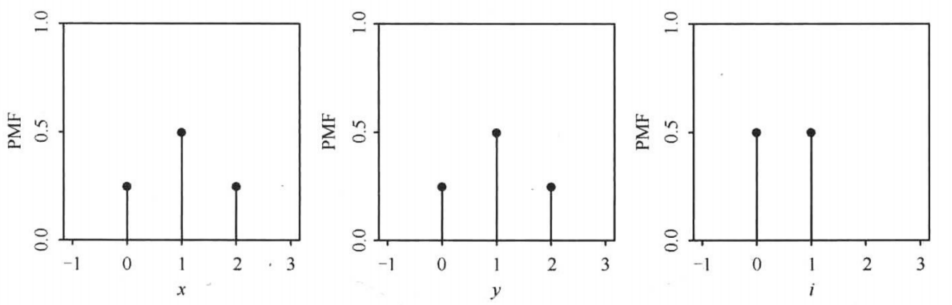
\includegraphics[width=12cm]{figures/Fig3.3.png}
	\end{figure}
\end{frame}

\begin{frame}{}
	\begin{exam}
		掷两颗骰子,其样本空间 $\Omega$ 含有 36 个等可能的样本点
		\begin{eqnarray*}
			\Omega=\{(x,y):x,y=1,2,\cdots,6\}
		\end{eqnarray*}
		令 $X$ 和 $Y$ 表示每个骰子分别出现的点数。试求下面随机变量的分布列: % 在 $\Omega$ 上定义如下三个随机变量,请给出其概率分布列
		\begin{enumerate}[<+-|alert@+>]
			\item $T_1:=X+Y=\mbox{骰子点数之和}$;
			\item $T_2:=14-(X+Y)$;
			\item $T_3:=\mbox{点数为 6 点的骰子的个数}$;
			\item $T_4:=\max\{X, Y\}=\mbox{骰子的最大点数}$
		\end{enumerate}

	\end{exam}
\end{frame}

\begin{frame}
	\begin{itemize}[<+-|alert@+>]
		\item $T_1, T_2$ 的概率分布列为 \pause
		      \begin{eqnarray*}
			      \left(\begin{array}{ccccccccccc}
				      2            & 3            & 4            & 5            & 6            & 7            & 8            & 9            & 10           & 11           & 12           \\
				      \frac{1}{36} & \frac{2}{36} & \frac{3}{36} & \frac{4}{36} & \frac{5}{36} & \frac{6}{36} & \frac{5}{36} & \frac{4}{36} & \frac{3}{36} & \frac{2}{36} & \frac{1}{36}
			      \end{array}\right)
		      \end{eqnarray*}
		      \pause
		      \begin{figure}[图 3.4.png]
			      \centering
			      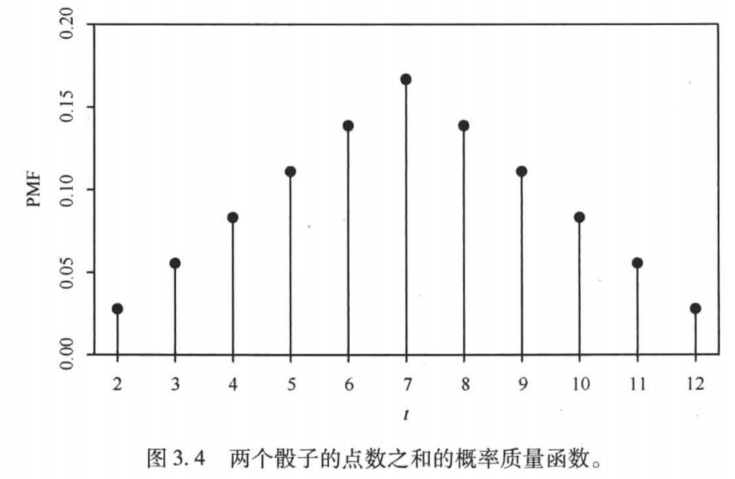
\includegraphics[width=9cm]{figures/Fig3.4.png}
		      \end{figure}

	\end{itemize}

\end{frame}

\begin{frame}
	\begin{itemize}[<+-|alert@+>]

		\item $T_3$ 的概率分布列为 \pause
		      \begin{eqnarray*}
			      \left(\begin{array}{ccc}
				      0             & 1             & 2            \\
				      \frac{25}{36} & \frac{10}{36} & \frac{1}{36}
			      \end{array}\right)
		      \end{eqnarray*}

		\item $T_4$ 的概率分布列为 \pause
		      \begin{eqnarray*}
			      \left(\begin{array}{cccccc}
				      1            & 2            & 3            & 4            & 5            & 6             \\
				      \frac{1}{36} & \frac{3}{36} & \frac{5}{36} & \frac{7}{36} & \frac{9}{36} & \frac{11}{36}
			      \end{array}\right)
		      \end{eqnarray*}
	\end{itemize}

\end{frame}

% \begin{frame}
%   \begin{exam}
%     设离散型随机变量的 $X$ 分布列为
%     \begin{eqnarray*}
%       \left(\begin{array}{ccc}
%               -1  &2 &3\\
%               0.25 & 0.5 & 0.25
%             \end{array}\right)
%     \end{eqnarray*}
%     试求 $P (X\le 0.5), P (1.5<X\le 2.5)$, 并写出 $X$ 的分布函数.
%   \end{exam}

%   \jieda $$P(X\le 0.5)=P(X=-1)=0.25,$$ $$P(1.5<X\le 2.5)=P(X=2)=0.5.$$

%   其分布函数为 \pause
%   \begin{eqnarray*}
%     F(x)=\left\{
%     \begin{array}{ll}
%       \pause  0, &  x<-1\\  \pause
%       \pause 0.25,& -1\le x<2\\  \pause
%       \pause  0.25+0.5=0.75,&  2\le x<3\\  \pause
%       \pause  0.25+0.5+0.25, & x\ge 3 \pause
%     \end{array}\right.
%   \end{eqnarray*}

% \end{frame}


%\subsection{连续型分布}

\begin{frame}
	\frametitle{连续型随机变量及分布}
	\begin{defi}[连续型随机变量] 设 $X$ 为一随机变量,$F (x)$ 为随机变量 $X$ 的分布函数,如果存在非负可积函数 $p (x)$ 使得
		\begin{eqnarray}\label{eq:contrvdist}
			F(x)=\int_{-\infty}^xp(y)dy
		\end{eqnarray}
		则称 $X$ 为连续型随机变量,其分布函数称之为连续型分布函数,函数 $p (x)$ 称为 $X$ 的概率密度函数,简称密度函数或密度.
	\end{defi}
	\pause
	\begin{rmk}
		\begin{itemize}[<+-|alert@+>]
			\item 能够表为 \eqref{eq:contrvdist} 式变上限积分的函数 $F (x)$ 在分析中称为绝对连续函数。绝对连续函数必为连续函数.
			\item 在若干个点上或零测集上改变密度函数 $p (x)$ 的值并不影响其积分的值,从而不影响分布函数 $F (x)$ 的值,这意味着连续分布的密度函数不唯一.
		\end{itemize}
	\end{rmk}

\end{frame}

\begin{frame}
	\frametitle{密度函数的性质}
	容易验证,随机变量 $X$ 的密度函数有以下性质
	\begin{enumerate}[<+-|alert@+>]
		\item 非负性:$p (x)\ge 0$;
		\item 正则性:$\int_{-\infty}^\infty p (x) dx=1$.
	\end{enumerate}

\end{frame}


\begin{frame}
	\frametitle{连续型随机变量分布的一些常见性质}
	\begin{itemize}
		\item $p(x)=F^\prime (x)$;
		\item $P(a< X\le b)=F(b)-F(a)=\int_a^bp(x)dx$;
		\item $0\le P (X=a)\le P (X\in (a-\epsilon,a))=\int_{a-\epsilon}^ap (x) dx\stackrel{\epsilon\rightarrow 0}{\longrightarrow} 0$, 故 $P (X=a)=0$,即连续型随机变量取值单点的概率为 0;
		\item $P(a<X\le b)=P(a\le X<b)=P(a\le X\le b)=P(a<X<b)$;
		\item 对任意的 Borel 集 $B$,
		      \begin{eqnarray*}
			      P(X\in B)=\int_Bp(x)dx
		      \end{eqnarray*}
		\item $P(X\in[x,x+\Delta x])=\int_x^{x+\Delta x}p(y)dy=p(\xi)\Delta x\approx p(x)\Delta x$
	\end{itemize}
\end{frame}
% \begin{frame}
%   \begin{exam}
%     向区间 $(0,a)$ 上任意投点,用 $X$ 表示这个点的坐标。设该点落在 $(0,a)$ 中任一小区间的概率与这个小区间的长度成正比,而与小区间的位置无关。求 $X$ 的分布函数及密度函数.
%   \end{exam}

%   \pause
%   \jieda 记 $X$ 的分布函数为 $F (x)$, 则
%   \begin{itemize}[<+-|alert@+>]
%   \item 当 $x<0$ 时,$\{X\le x\}$ 为不可能事件,故 $F (x)=P (X\le x)=0$;
%   \item 当 $x\ge a$ 时,$\{X\le x\}$ 是必然事件,故 $F (x)=P (X\le x)=1$;
%   \item 当 $x\in [0,a)$ 时, 有 $F (x)=P (X\le x)=P (0\le X\le x)=kx$, 其中 $k$ 为比例系数.
%   \item 注意到 $1=F (a)=P (0\le X\le a)=ka$, 故 $k=1/a$
%   \end{itemize}
%   \pause
%   故 $X$ 的分布函数为
%   \pause
%   \begin{eqnarray*}
%     F(x)=\left\{
%     \begin{array}{ll}
%       0,& x<0\\
%       x/a, & 0\le x<a\\
%       1,& x\ge a
%     \end{array}
%           \right.
%   \end{eqnarray*}
% \end{frame}
% \begin{frame}
%   下面我们求 $X$ 的密度函数,
%   \begin{itemize}
%   \item 当 $x<0$ 或 $x>a$ 时, $p (x)=F^\prime (x)=0$;
%   \item 当 $0<x<a$ 时,$p (x)=F^\prime (x)=1/a$;
%   \item 当 $x=0,a$ 时,$p (x)$ 可取任意值,一般就近取值为宜,不会影响概率的计算.
%   \end{itemize}
%   故 $X$ 的密度函数为
%   \begin{eqnarray*}
%     p(x)=\left\{
%     \begin{array}{ll}
%       1/a,&0<x<a,\\
%       0,&\mbox{其他}.
%     \end{array}
%           \right.
%   \end{eqnarray*}
%   其密度函数也可取为
%   \begin{eqnarray*}
%     p(x)=\left\{
%     \begin{array}{ll}
%       1/a,&0\le x\le a,\\
%       0,&\mbox{其他}.
%     \end{array}
%           \right.
%   \end{eqnarray*}

% \end{frame}

% \begin{frame}
%   \begin{exam}
%     某种型号电子元件的寿命 $X$(以小时计) 具有以下概率密度函数
%     \begin{eqnarray*}
%       p(x)=\left\{
%       \begin{array}{ll}
%         k/x^2,&x>1000,\\
%         0,&\mbox{其他}.
%       \end{array}
%             \right.
%     \end{eqnarray*}
%     其中 $k$ 为未知常数。现有一大批此种元件 (设各元件工作相互独立),问
%     \begin{enumerate}
%     \item 任取 1 只,其寿命大于 1500 小时的概率是多少?
%     \item 任取 4 只,4 只寿命都大于 1500 小时的概率是多少?
%     \item 任取 4 只,至少有一只寿命大于 1500 小时的概率是多少?
%     \item 若已知一只元件寿命大于 1500 小时,则该元件寿命大于 2000 小时的概率是多少?
%     \end{enumerate}

%   \end{exam}
% \end{frame}
%\subsection{其他类型分布}

\begin{frame}{一个连续型随机变量的例子}
\begin{exam}
  考虑概率空间$(\Omega,\mathcal{F}, P)$, 其中$\Omega:=[0,1], \mathcal{F}:=\mathcal{B}([0,1])$, $P(A):=m(A)$即$A$的Lebesgue测度. 定义
  \[\theta(\omega)=\omega, \ \forall \omega\in [0,1].\]
  \pause 显然, $\theta(\omega)$是随机变量, 且其分布函数为\pause
  \begin{eqnarray*}
	F(x)=P(\theta(\omega)\leq x)=\left\{
		\begin{array}{ll}
		 0, & x<0,\\
		 x, & 0\leq x<1\\
		 1, & x\geq 1.
		\end{array}
		\right.
  \end{eqnarray*}
其分布密度为
\[p(x)=F'(x)=1, x\in (0,1).\]

\end{exam}


\end{frame}







\begin{frame}
	\begin{exam}
		定义函数 $F (x)$ 如下
		\begin{eqnarray*}
			F(x)=\left\{
			\begin{array}{ll}
				0,              & x< 0,      \\
				\dfrac{1+x}{2}, & 0\le x< 1, \\
				1,              & x\ge 1.
			\end{array}
			\right.
		\end{eqnarray*}
		试说明  \begin{enumerate}
			\item $F (x)$ 为分布函数;
			\item $F (x)$ 既非离散型也非连续型分布;
			\item $F (x)$ 可分解为
			      \begin{eqnarray*}
				      F(x)=\frac{1}{2}F_1(x)+\frac{1}{2}F_2(x)
			      \end{eqnarray*}
			      \pause  其中 \begin{eqnarray*}
				      F_1(x)=\left\{
				      \begin{array}{ll}
					      0, & x< 0,    \\
					      1, & x\ge 0.
				      \end{array}
				      \right.
				      \quad  F_2(x)=\left\{\begin{array}{ll}
					      0, & x<0,       \\
					      x, & 0\le x< 1, \\
					      1, & x\ge 1.
				      \end{array}
				      \right.
			      \end{eqnarray*}
		\end{enumerate}

	\end{exam}
\end{frame}


\begin{frame}
	\frametitle{勒贝格分解}
	\begin{thm}[勒贝格分解] 对任一分布函数 $F (x)$ 有如下分解
		\begin{eqnarray*}
			F(x)=c_1F_1(x)+c_2F_2(x)+c_3F_3(x),
		\end{eqnarray*}
		其中常数 $c_1,c_2,c_3\ge 0, c_1+c_2+c_3=1,$ 而 $F_1 (x),F_2 (x),F_3 (x)$ 都是分布函数,$F_1 (x)$ 为纯跳跃离散型函数,$F_2 (x)$ 为连续型分布函数,$F_3 (x)$ 为奇异型分布函数(见教材3.6节奇异连续型分布构造).
	\end{thm}
	\vspace{0.3cm}
	\pause
	\begin{itemize}[<+-|alert@+>]
		\item 上述定理中奇异函数的含义及定理的证明可参见一般的实变函数论教科书,这里我们不再详述,仅指出几种特殊情况:
		      \begin{itemize}
			      \item 在分解式中取 $c_1=1,c_2=c_3=0$ 便得到我们所讨论的离散型分布函数;
			      \item 在分解式中取 $c_2=1,c_1=c_3=0$ 便得到连续型分布函数;
			      \item 若取 $c_3=0, c_1\neq 0, c_2\neq 0, c_1+c_2=1$ 便得到离散与连续混合分布
		      \end{itemize}
		\item 从上面分析可看出,随机变量除了离散型与连续型外还有很多其他类型.
	\end{itemize}

\end{frame}


\subsection{随机变量的存在性}

 \begin{frame}{分布函数与随机变量}
 \begin{align*}
 &	\left. \begin{array}{c}
		 (\Omega, \mathcal{F}, P) \\
		  \\
		 X(\omega)
			\end{array}\right\}\Rightarrow\pause P(X\leq x)=: F(x)\pause	\Rightarrow  \left\{\begin{array}{l}
		   \mbox{单调非降性} \\
		   \mbox{右连续性}\\
		   \mbox{规范性}
		\end{array}\right. \\
 \pause
 \\
 \\
 &\left.\begin{array}{r}
	 \mbox{单调非降性} \\
	 \mbox{右连续性}\\
	 \mbox{规范性}
 \end{array}\right\}\mbox{的} F (x) \mbox{给定}\Rightarrow\pause \mbox{存在}  \left\{\begin{array}{l}
		 (\Omega, \mathcal{F}, P) \\
		 \\
		 X(\omega)
	 \end{array}\right. \mbox{使得} F (x)=P (X\leq x) ?
 \end{align*}


 \end{frame}

 \begin{frame}{随机变量的存在性问题分析}
 %	由前面所学知识易知:给定一个随机变量,我们可定义其分布函数,并且分布函数具有性质:单调非降,右连续,$F (-\infty)=0$, $F (+\infty)=1$. 那么反过来呢?
 %	\pause \begin{prob}
 %		给定一个分布函数 $F (x)$, 即函数 $F (x)$ 具有分布函数的性质:单调非降,右连续,$F (-\infty)=0$, $F (+\infty)=1$, 是否一定存在一个概率空间 $(\Omega,\mathcal{F},P)$ 及其上的随机变量 $X$ 使得其分布函数恰为 $F (x)$?
 %	\end{prob}
 %	\pause
 \begin{thm}\label{sec:existofrv}
 \hspace{-0.2cm} 若 $F (x)$ 是右连续、单调非降函数,且 $F (-\infty)=0, F (+\infty)=1$, 则存在一个概率空间 $(\Omega,\mathcal{F},P)$ 及其上的随机变量 $X (\omega)$, 使 $X (\omega)$ 的分布函数恰好是 $F (x)$.
 \end{thm}

 \textcolor{cyan}{分析:}
 \begin{itemize}[<+-|alert@+>]
	 %\item 取 $\Omega=[0,1]$, $\mathcal{F}$ 为 $[0,1]$ 上的 Borel 集全体,取 $P$ 为直线上的 Lebesgue 测度 (是长度概念的推广,但对一切 Borel 集有定义);
	 \item 对 $[0,1]$ 上的均匀分布随机变量 $\theta (\omega)=\omega$, 其分布函数为 % 有 %, 其分布函数 % 则 $\theta (\omega)$ 是 $(\Omega,\mathcal{F},P)$ 上的随机变量,并且,,
	 \begin{eqnarray*}
		 P(\theta(\omega)\le x)=P(\omega\in[0,x])=x, \ \forall x\in[0,1];
	 \end{eqnarray*}
	 \item $F (x)\in[0.1]$, 若将上式中的 $x$ 替换为 $F (x)$, 则有
		 \begin{eqnarray*}
		 P(\theta(\omega)\le F(x))=F(x);
	 \end{eqnarray*}
	 \item 若分布函数 $F (x)$ 可逆,则
	 \begin{eqnarray*}
	 P(F^{-1}(\theta(\omega))\le x)=	P(\theta(\omega)\le F(x))=\pause F(x);
	 \end{eqnarray*}

	 \item 考虑 $X (\omega):=F^{-1}(\theta (\omega))$, 则 $F_X (x)= P (F^{-1}(\theta (\omega))\le x)= F (x)$;

 %    \item $F (x)$\textcolor{red}{不一定可逆}, 能否定义一种映射 $G$ 使得
 %    \[\{\theta(\omega)\le F(x)\}=\{G(\theta(\omega))\le x\}?\]

 \end{itemize}


 \end{frame}
 \begin{frame}{随机变量的存在性问题分析}
	 \begin{itemize}[<+-|alert@+>]
	 \item $F (x)$\textcolor{red}{不一定可逆}, 能否定义一个函数 $G$ 使得
		 \[\{\theta(\omega)\le F(x)\}=\{G(\theta(\omega))\le x\}?\]
	 \item 上述等式也即寻求如下等价性
	 \[G(\theta)\leq x \Leftrightarrow F(x)\ge \theta \]
	 \item 因此,若函数 $G$ 存在,则对任意给定的 $\theta$ 必须满足
	 \[G(\theta)\leq x, \quad  \forall x\in \{x: F(x)\ge\theta\}\]
	 \item 故所寻找的函数 $G$ 需有以下性质
	 \[G(\theta)\leq \inf\{x:F(x)\geq \theta\}\]
	 \item 上述不等式右侧的下确界也是 $G$ 的一种选择,可以证明选此下确界作为函数 $G$ 的定义的确具有我们所要求的性质.%,
	 \end{itemize}




 \end{frame}

 \begin{frame}{单调逆 (一般逆) 的定义}
	 \vspace{-0.1cm}
	 \begin{defi}
		 设 $F (x)$ 是右连续、单调非降函数,且 $F (-\infty)=0, F (+\infty)=1$. 对任意的 $p\in (0,1)$, 我们称
		 \begin{eqnarray*}
			 F^{-1}(p):=\inf\{x: F(x)\geq p\}, %\forall p\in (0,1),
		 \end{eqnarray*}
		 为函数 $F (x)$ 的单调逆或一般逆.
	 \end{defi}

 \pause
 \begin{rmk} \ 	 $F^{-1}(p)$ 在概率论中也称为函数 $F (x)$ 的 $p$ 分位数函数或与其相对应的随机变量 $X$ 的 $p$ 分位数,通常用 $x_p$ 或 $\xi_p$ 来表示.
 \end{rmk}
 \begin{thm}
	 设 $F (x), F^{-1}(p)$ 定义如上,则
	 \[F^{-1}(p)\leq x \Leftrightarrow F(x)\ge p \]
 \end{thm}
 \pause
 \zheng 令 $A:=\{y: F (y)\geq p\}$, 则 \pause
 \begin{itemize}[<+-|alert@+>]
	 \item $\Leftarrow$: $F (x)\geq p$ 蕴含 \pause $F^{-1}(p):=\inf A\leq x$\pause
	 \item $\Rightarrow$: $F^{-1}(p)\leq x$ 即 $x\geq F^{-1}(p):=\inf A=:x_0$\pause
	 \begin{itemize}[<+-|alert@+>]
		 \item 若 $x_0\in A$, 则显然 \pause $F (x)\geq F (x_0)\geq p$\pause
		 \item 若 $x_0\notin A$, 则存在 \pause $\{x_n\}_{n\geq 1}\subset A$ 使得 $x_n>x_0$ 且 $\lim_{n\rightarrow \infty} x_n=x_0$,\pause  从而 \pause
		 \[F(x)\geq F(x_0)=F(\lim_{n\rightarrow \infty}x_n)=\pause \lim_{n\rightarrow \infty}F(x_n)\geq\pause p;\]
	 \end{itemize}
 \end{itemize}
 \end{frame}
 \begin{frame}{随机变量存在性的证明}
 \trc{定理 \ref{sec:existofrv} 的证明:}\pause
 \begin{itemize}[<+-|alert@+>]
	 \item 取 $\Omega=[0,1]$, $\mathcal{F}$ 为 $[0,1]$ 上的 Borel 集全体,取 $P$ 为直线上的 Lebesgue 测度 (是长度概念的推广,但对一切 Borel 集有定义);
	 \item 定义: $\theta (\omega)=\omega$, 则 $\theta (\omega)$ 是 $(\Omega,\mathcal{F},P)$ 上的随机变量,并且,对一切的 $0\le x\le 1$,
	 \begin{eqnarray*}
		 P(\theta(\omega)\le x)=P(\omega\in[0,x])=x;
	 \end{eqnarray*}
	 \item 考虑 $X (\omega):=F^{-1}(\theta (\omega))$, 则
	{\small\begin{eqnarray*}
			 F_X(x)=P(X\le x)=\pause P(F^{-1}(\theta(\omega))\le x)\pause \xlongequal[p\le F(x)]{F^{-1}(p)\le x} P(\theta(\omega)\le F(x))=\pause F(x)
	 \end{eqnarray*}}


 \end{itemize}


 \end{frame}



 %\begin{frame}
 %	\frametitle{随机变量的 $p$ 分位数函数}
 %	\vspace{-0.3cm}
 %	\begin{defi}
 %		设 $X$ 是概率空间 $(\Omega,\mathcal{F},P)$ 上的随机变量,$F (x)$ 为其分布函数。对于 $p\in (0,1)$, 定义
 %		\begin{eqnarray*}
 %			F^{-1}(p):=\sup\{x:F(x)<p\}\pause =\inf\{x: F(x)\geq p\}.
 %		\end{eqnarray*}
 %		称 $F^{-1}(p)$ 为 $F$ 或 $X$ 的 $p$ 分位数,通常用 $x_p$ 或 $\xi_p$ 来表示.
 %	\end{defi}
 %
 %
 %\end{frame}
 \begin{frame}
	 \frametitle{单调逆 (一般逆) 的性质}

	 \begin{itemize}[<+-|alert@+>]
		 \item $F^{-1}(F (x))\leq x, \forall x\in R$ :\pause\  设 $x_0\in R$ 任意给定且 $F (x_0)=p_0$, 则 \pause
		 \begin{align*}
		  F^{-1}(F(x_0))&=\pause F^{-1}(p_0)=\pause \inf\{x: F(x)\geq p_0\}\\
		  &=\pause \inf\{x: F(x)\geq F(x_0)\}\leq\pause  x_0
		 \end{align*}
		 \item $F (F^{-1}(p))\geq p, \forall p\in (0,1)$:\pause 设 $p_0\in (0,1)$ 任意给定且
		 \begin{align*}
		 F^{-1}(p_0)=x_0=\inf\{x: F(x)\geq p_0\}=:\inf A, %
		 \end{align*}
	 \begin{itemize}[<+-|alert@+>]
		 \item 若 $x_0\in A$, 则显然有 $F (F^{-1}(p_0))=F (x_0)\geq p_0$;
		 \item 若 $x_0\notin A$, 则 \pause 存在 $\{x_n\}_{n\geq 1}\subset A$ 使得 $x_n>x_0$ 且 $\lim_{n\rightarrow \infty} x_n=x_0$,\pause  从而由函数 $F (x)$ 的右连续性可知 \pause
		 \[F(F^{-1}(p_0))=F(x_0)=F(\lim_{n\rightarrow \infty}x_n)=\pause \lim_{n\rightarrow \infty}F(x_n)\geq\pause p_0;\]
	 \end{itemize}
	 \item $F^{-1}(p)$ 关于 $p$ 单调非降:集合 $\{x:F (x)\geq p\}$ 关于 $p$ 单调不增,故其下确界也关于 $p$ 单调非降
		 \end{itemize}
	 \end{frame}

 \begin{frame}
	 \frametitle{单调逆 (一般逆) 的性质}
	 下面的几条性质 %,\trc{(留做作业)}
	 \begin{itemize}[<+-|alert@+>]
		 \item  $F^{-1}(p)$ 关于 $p$ 是左连续的;
		 \item $F^{-1}(p):=\inf\{x: F(x)\geq p\}=\sup\{x:F(x)<p\}$
		 \item $x<F^{-1}(p)\Leftrightarrow F(x)<p$
		 %\item $F (x)<p$, 则 $x<F^{-1}(p)$
	 \end{itemize}

 \end{frame}

 \begin{frame}{思考}
	 若 $F (x)$ 是左连续、单调非降函数,且 $F (-\infty)=0, F (+\infty)=1$, 是否存在一个概率空间 $(\Omega,\mathcal{F},P)$ 及其上的随机变量 $X (\omega)$, 使得
	 \[F(x)=P(X<x).\]



 \end{frame}
